\section{Fusing Query Variations}
Despite the infrequent occurrences, it is evident from the data presented in \fig{fig:dist-plots} that, in some instances, superior performance is observed for the query variations over their original counterparts. This is shown by a positive nDCG@10 $\Delta$. Following the original research, this phenomenon is the impetus for exploring the amalgamation of different query variation types.

The resulting effectiveness of merging the rankings for each variation category is illustrated in \tab{tab:ant-fusion-table}, \tab{tab:trec-fusion-table}, and \tab{tab:typo-fusion-table}. Rows denoted as $ RFC_C $ signify the amalgamation of results derived from query variations obtained by applying $ M_C $ methods using the Reciprocal Rank Fusion (RRF) technique, while $ RFC_{All} $ encompasses the results from all query variation methods. It is notable that the $ RFC_{Ordering} $ category is excluded, as it comprises only a single method.

\subsection{Research Question 1: Reproduction}
\begin{table}[ht]
\centering
\caption{Effectiveness (nDCG@10) of different methods for ANTIQUE when employing rank fusion (RRF) of the rankings obtained by using different sets of queries.}
\label{tab:ant-fusion-table}
\begin{tabularx}{\columnwidth}{l|X|X|X|X|X|X|X}
\textbf{} & \textbf{BM25} & \textbf{RM3} & \textbf{KNRM} & \textbf{CKNRM} & \textbf{EPIC} & \textbf{BERT} & \textbf{T5} \\ \hline
Original Query   & 0.2286 & 0.217  & 0.2182  & 0.2065 & 0.266  & 0.3947  & 0.3333 \\ \hline
$RRF_{Misspelling}$ & 0.1714 & 0.1653 & 0.1804  & 0.1664 & 0.2065 & 0.2675  & 0.2441 \\
$RRF_{Naturality}$  & 0.1842 & 0.1865 & 0.2058  & 0.2039 & 0.2407 & 0.3002  & 0.271  \\
$RRF_{Paraphrase}$  & 0.1924 & 0.1861 & 0.1955  & 0.1765 & 0.2401 & 0.3223  & 0.2894 \\
$RRF_{Synonym}$     & 0.1831 & 0.177  & 0.2009  & 0.1847 & 0.2184 & 0.2944  & 0.2678 \\
$RRF_{All}$         & 0.2076 & 0.206  & 0.219   & 0.2121 & 0.2547 & 0.3197  & 0.2867 \\ \hline
Best Query       & 0.4149 & 0.2716 & 0.2836  & 0.3369 & 0.3019 & 0.3981  & 0.3911
\end{tabularx}%
\end{table}

\begin{table}[ht]
\centering
\caption{Effectiveness (nDCG@10) of different methods for TREC-DL-2019 when employing rank fusion (RRF) of the rankings obtained by using different sets of queries.}
\label{tab:trec-fusion-table}
\begin{tabularx}{\columnwidth}{l|X|X|X|X|X|X|X}

\textbf{} & \textbf{\textbf{BM25}} & \textbf{\textbf{RM3}} & \textbf{KNRM} & \textbf{CKNRM} & \textbf{EPIC} & \textbf{BERT} & \textbf{T5} \\ \hline
Original Query   & 0.4795 & 0.5156 & 0.4941 & 0.4931 & 0.624  & 0.6358 & 0.6998 \\ \hline
$RRF_{Misspelling}$ & 0.3035 & 0.3073 & 0.3175 & 0.3175 & 0.3838 & 0.3941 & 0.4636 \\
$RRF_{Naturality}$  & 0.4744 & 0.4972 & 0.4668 & 0.464  & 0.5925 & 0.6005 & 0.6643 \\
$RRF_{Paraphrase}$  & 0.4742 & 0.4865 & 0.4883 & 0.433  & 0.5847 & 0.577  & 0.6616 \\
$RRF_{Synonym}$     & 0.4247 & 0.4066 & 0.4117 & 0.4048 & 0.4975 & 0.4902 & 0.5632 \\
$RRF_{All}$         & 0.4752 & 0.4958 & 0.4965 & 0.4951 & 0.5908 & 0.5939 & 0.6442 \\ \hline
Best Query       & 0.6964 & 0.5401 & 0.6116 & 0.6983 & 0.6939 & 0.6784 & 0.7598
\end{tabularx}
\end{table}

The incorporation of RRF yields significant enhancements in nDCG@10, as demonstrated in \tab{tab:ant-fusion-table} and \tab{tab:trec-fusion-table}. A comparative analysis with \tab{tab:ant-main-table} and \tab{tab:trec-main-table} reveals that, in numerous instances, the outcomes are either on par with or surpass the performance achieved through the sole utilisation of query variations. This pattern of results aligns with the original study's findings, bolstering the assertion that RRF can augment retrieval effectiveness. However, the augmentation by RRF does not consistently outperform the retrieval outcomes associated with the unaltered original queries. This observation underscores the nuanced impact of RRF within the context of query variations and retrieval performance.

\subsection{Research Question 2: Expansion}
\begin{table}[ht]
\centering
\caption{Effectiveness (nDCG@10) of different methods for DL-TYPO when employing rank fusion (RRF) of the rankings obtained by using different sets of queries.}
\label{tab:typo-fusion-table}
\begin{tabularx}{\columnwidth}{l|X|X|X|X|X|X|X}

\textbf{} & \textbf{BM25} & \textbf{RM3} & \textbf{KNRM} & \textbf{CKNRM} & \textbf{EPIC} & \textbf{BERT} & \textbf{T5} \\ \hline
Original Query   & 0.1911 & 0.1757 & 0.1994 & 0.1798 & 0.1862 & 0.1951 & 0.2882 \\ \hline
$RRF_{Misspelling}$ & 0.0979 & 0.0933 & 0.1147 & 0.0855 & 0.1006 & 0.0782 & 0.1373 \\
$RRF_{Naturality}$  & 0.1657 & 0.154  & 0.1592 & 0.1498 & 0.161  & 0.1557 & 0.2277 \\
$RRF_{Paraphrase}$  & 0.1965 & 0.1919 & 0.1839 & 0.1722 & 0.202  & 0.1931 & 0.2479 \\
$RRF_{Synonym}$     & 0.0883 & 0.0795 & 0.1214 & 0.0945 & 0.1051 & 0.0932 & 0.1477 \\
$RRF_{All}$         & 0.1546 & 0.1516 & 0.184  & 0.159  & 0.1656 & 0.156  & 0.2098 \\ \hline
Best Query        & 0.3156 & 0.3024 & 0.275  & 0.317  & 0.3052 & 0.2913 & 0.421 
\end{tabularx}
\end{table}


The effectiveness results (nDCG@10) for DL-TYPO when employing RRF are depicted in \tab{tab:typo-fusion-table}. They exhibit a noticeable disparity compared to the outcomes from ANTIQUE and TREC-DL-2019, as shown in \tab{tab:trec-fusion-table} and \tab{tab:typo-fusion-table}. DL-TYPO demonstrates lower nDCG@10 values for the original queries, indicative of a more challenging retrieval scenario. The influence of query variations and their subsequent amalgamation through RRF mirrors the results in ANTIQUE and TREC-DL-2019, as they lead to enhancements over the original queries. Nonetheless, these improvements are more modest in DL-TYPO, underscoring the unique characteristics of the dataset and the incredible difficulty in achieving substantial enhancements through query variations and RRF.

This disparity arises from the inherently more challenging nature of queries in the DL-TYPO dataset, which contain typos, resulting it it showing lower retrieval effectiveness. Consequently, the improvements stemming from query variations and RRF are less pronounced than in ANTIQUE and TREC-DL-2019. The disparities in results underscore the dataset-specific nature of this research and emphasise the significance of considering the distinct attributes and challenges of different datasets when exploring query variations and their impact on retrieval performance.

\subsection{Query Variations Performance}
\begin{figure}
    \centering
    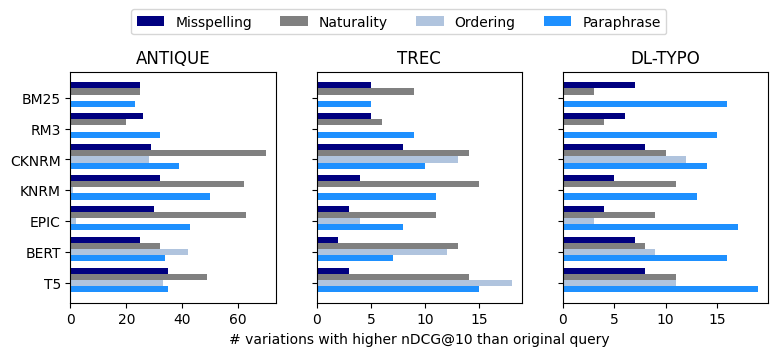
\includegraphics[width=1\linewidth]{5Results/fusion/plot_pos_diffs.png}
    \caption{Number of variations with higher effectiveness (nDCG@10) than original query per model for each variation category.}
    \label{fig:pos-diffs}
\end{figure}

\fig{fig:pos-diffs} provides visual insight into the performance of various query variation methods. The naturality and paraphrase methods exhibit more substantial improvements in variation effectiveness over the original queries compared to the other methods. Notably, the paraphrase category boasts the highest number of variations, demonstrating improved effectiveness across all models and datasets. This implies that paraphrasing query variations can outperform the original queries. The counts of such improvements range from 13 to 19, highlighting significant variability in successful paraphrased queries across models and datasets. This variance can be attributed to the propensity of paraphrasing methods to enhance queries by rectifying spelling errors (e.g. See \secn{sec:novelFindings}) and replacing words with more appropriate synonyms (e.g. "real gohst pics" to "authentic gohst pics" through WordEmbedSynSwap).

In contrast, the ordering category exhibits limited variations with improved effectiveness. In some instances, such as Trad and NN on specific datasets like TREC-DL-2019 and ANTIQUE, no variations surpass the effectiveness of the original query. This can be attributed to the impact of alterations in word order on retrieval effectiveness, especially within traditional bag-of-words models. Overall, the data underscores the significance of the specific nature of query variations and their interaction with diverse retrieval models and datasets. Overall, paraphrasing variations show great promise in enhancing retrieval performance while ordering variations seem to have a restricted impact.

The data underscores the disparities in the effectiveness of query variations, particularly in DL-TYPO compared to ANTIQUE and TREC-DL-2019. DL-TYPO exhibits fewer variations with higher nDCG@10 effectiveness than the original query. This suggests that query variations have a less pronounced impact on retrieval effectiveness in DL-TYPO. The variability in the number of improvements is also conspicuous across the categories of query variations. Moreover, this variability depends on the specific retrieval model employed, with some models showing a more substantial number of successful query variations than others. These differences underscore the challenges posed by real-world queries containing typos in the DL-TYPO dataset, as opposed to the synthetic data in other datasets. These observations emphasise the need for further research to comprehend the unique challenges presented by diverse datasets when working with query variations and retrieval models.